\section{The Need for an Upgraded Forward Muon System}
\label{sec:nsw_motivation}

The luminosity increases planned to take place during Run 3 and the HL-LHC
era means that ATLAS will be subjected to exceedingly high particle rates.
As mentioned previously, the peak number of interactions per bunch-crossing observed during
Run 2 operations was $\langle \mu \rangle \approx 60$.
Given the recent experience of the LHC delivering above expectation,
the increases in collision intensity planned for Run 3 imply a peak number approaching
$\langle \mu \rangle \approx 80-100$. 
That of the HL-LHC, nearing luminosities of $10^{35}$\,cm$^{-2}$s$^{-1}$, implies peaks approaching $\langle \mu \rangle \approx 200$ or more, depending
on the beam configuration.
While most of the detectors in the ATLAS muon system were designed with large enough safety margins
to handle the foreseen rates, the inner-most forward station --- the Small Wheel --- will
exceed its design capabilities.
The current Small Wheel covers $1.0 < \lvert \eta \rvert < 2.7$ (Figure~\ref{fig:muon_plan_view_eta}).
At $\lvert \eta \rvert = \pm 2.7$, rates of $\approx 20$\,kHz/cm$^2$ are expected, far higher
than what the currently-installed MDT and CSC detectors and readout electronics can handle.
Moreover, the end-cap region of ATLAS covers nearly 63\% of the ATLAS muon system rapidity.
High detector performance in this region, therefore, is of the utmost importance in order to
achieve the long-term physics goals of ATLAS and the upgraded LHC.

The end-cap Level-1 muon trigger logic is based on track segments formed by hits in the TGC chambers
in the middle muon station at $z\approx 13$\,m, the first `Big Wheel' (Figure~\ref{fig:muon_plan_view_eta}).
The \pT~of muon candidates, used to define the thresholds at which the triggers accept an event, is
determined by the angle of the track segment with respect to the direction pointing back to the IP.
In the forward region of ATLAS there is a significant background rate composed of low energy particles ---
mainly protons, neutrons, and photons --- generated as a result of material interactions between
the Small and Big Wheels.
Figure~\ref{fig:cavern_bkg} illustrates the levels of material interactions within the ATLAS
cavern that lead to this so-called `cavern background'.
These low energy particles can produce `fake' triggers by traversing the end-cap chambers
at angles similar to that of real high-\pT~muons originating from the IP.
This situation is illustrated in Figure~\ref{fig:l1mu_rates}, wherein it is seen that
a significant fraction of the reconstructed muons in the forward muon system cannot be matched
to a trigger candidate from the ID.
These `fake' triggers amount to roughly 90\% of the total muon triggers in ATLAS.
With the foreseen luminosity upgrades of the LHC, the number of such triggers in the end-cap region
will exceed the \textit{total} ATLAS Level-1 trigger rate budget of 100\,kHz (only 20\,kHz are budgeted
for Level-1 muon triggers).

\begin{figure}[!htb]
    \begin{center}
        %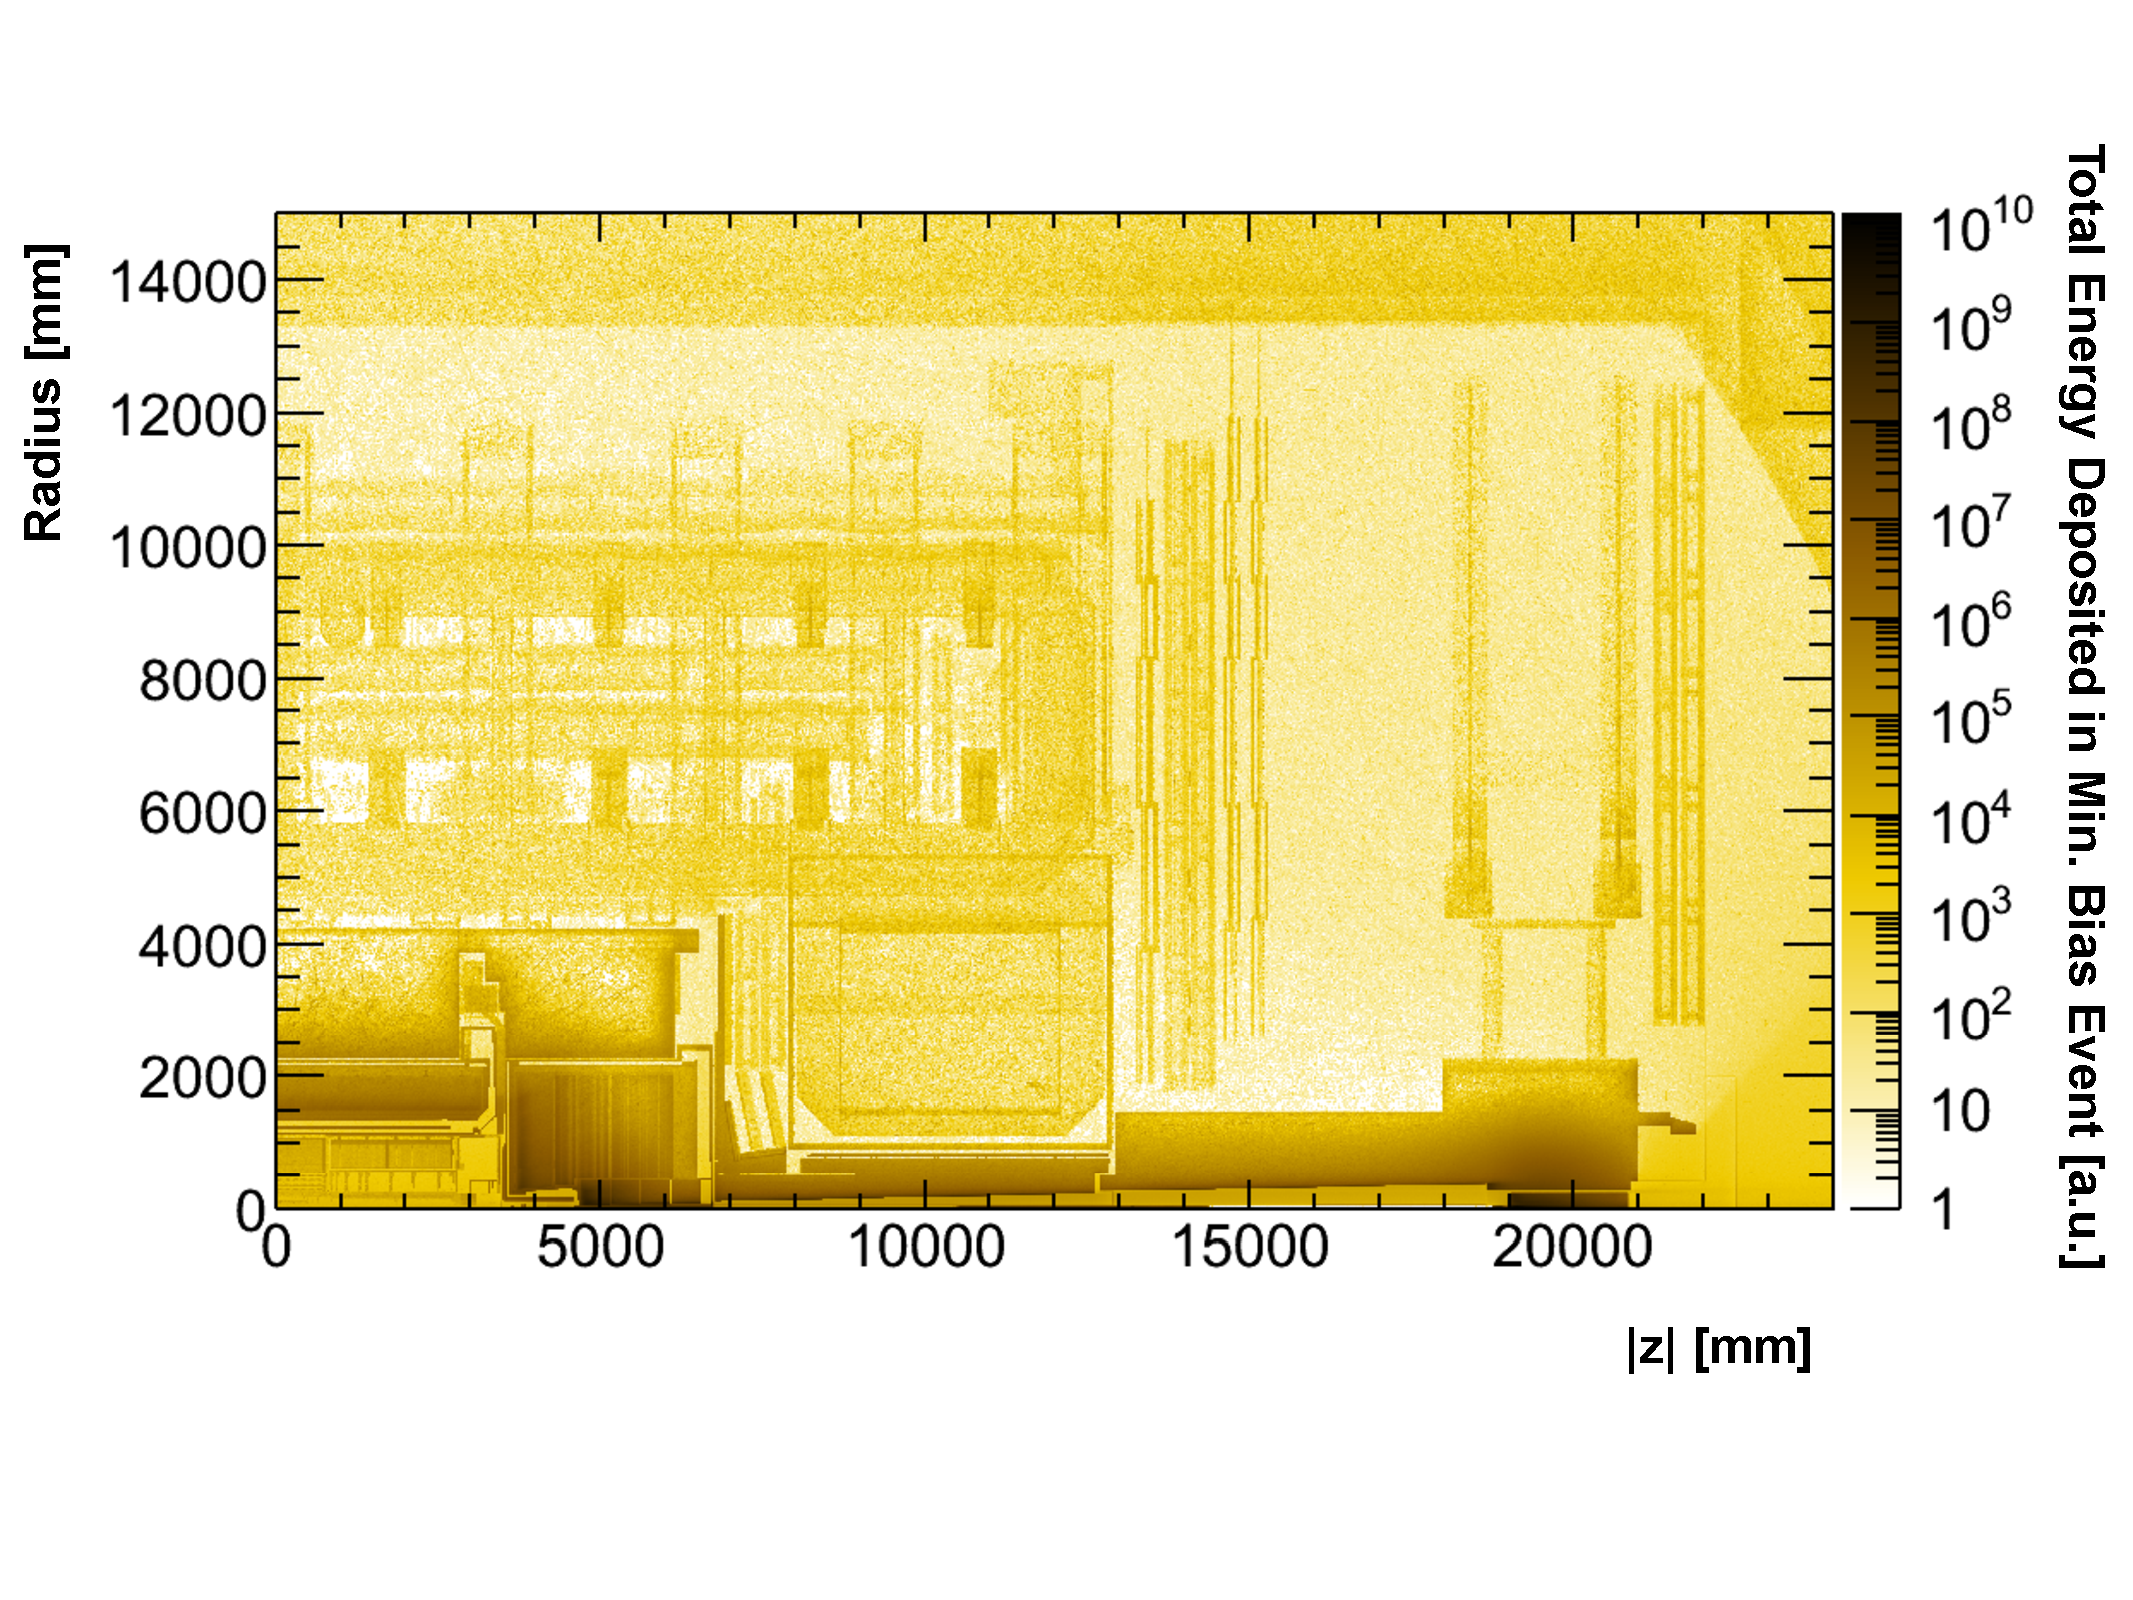
\includegraphics[width=0.8\textwidth]{figures/nsw/atlas_cavern_bkgPDF}
        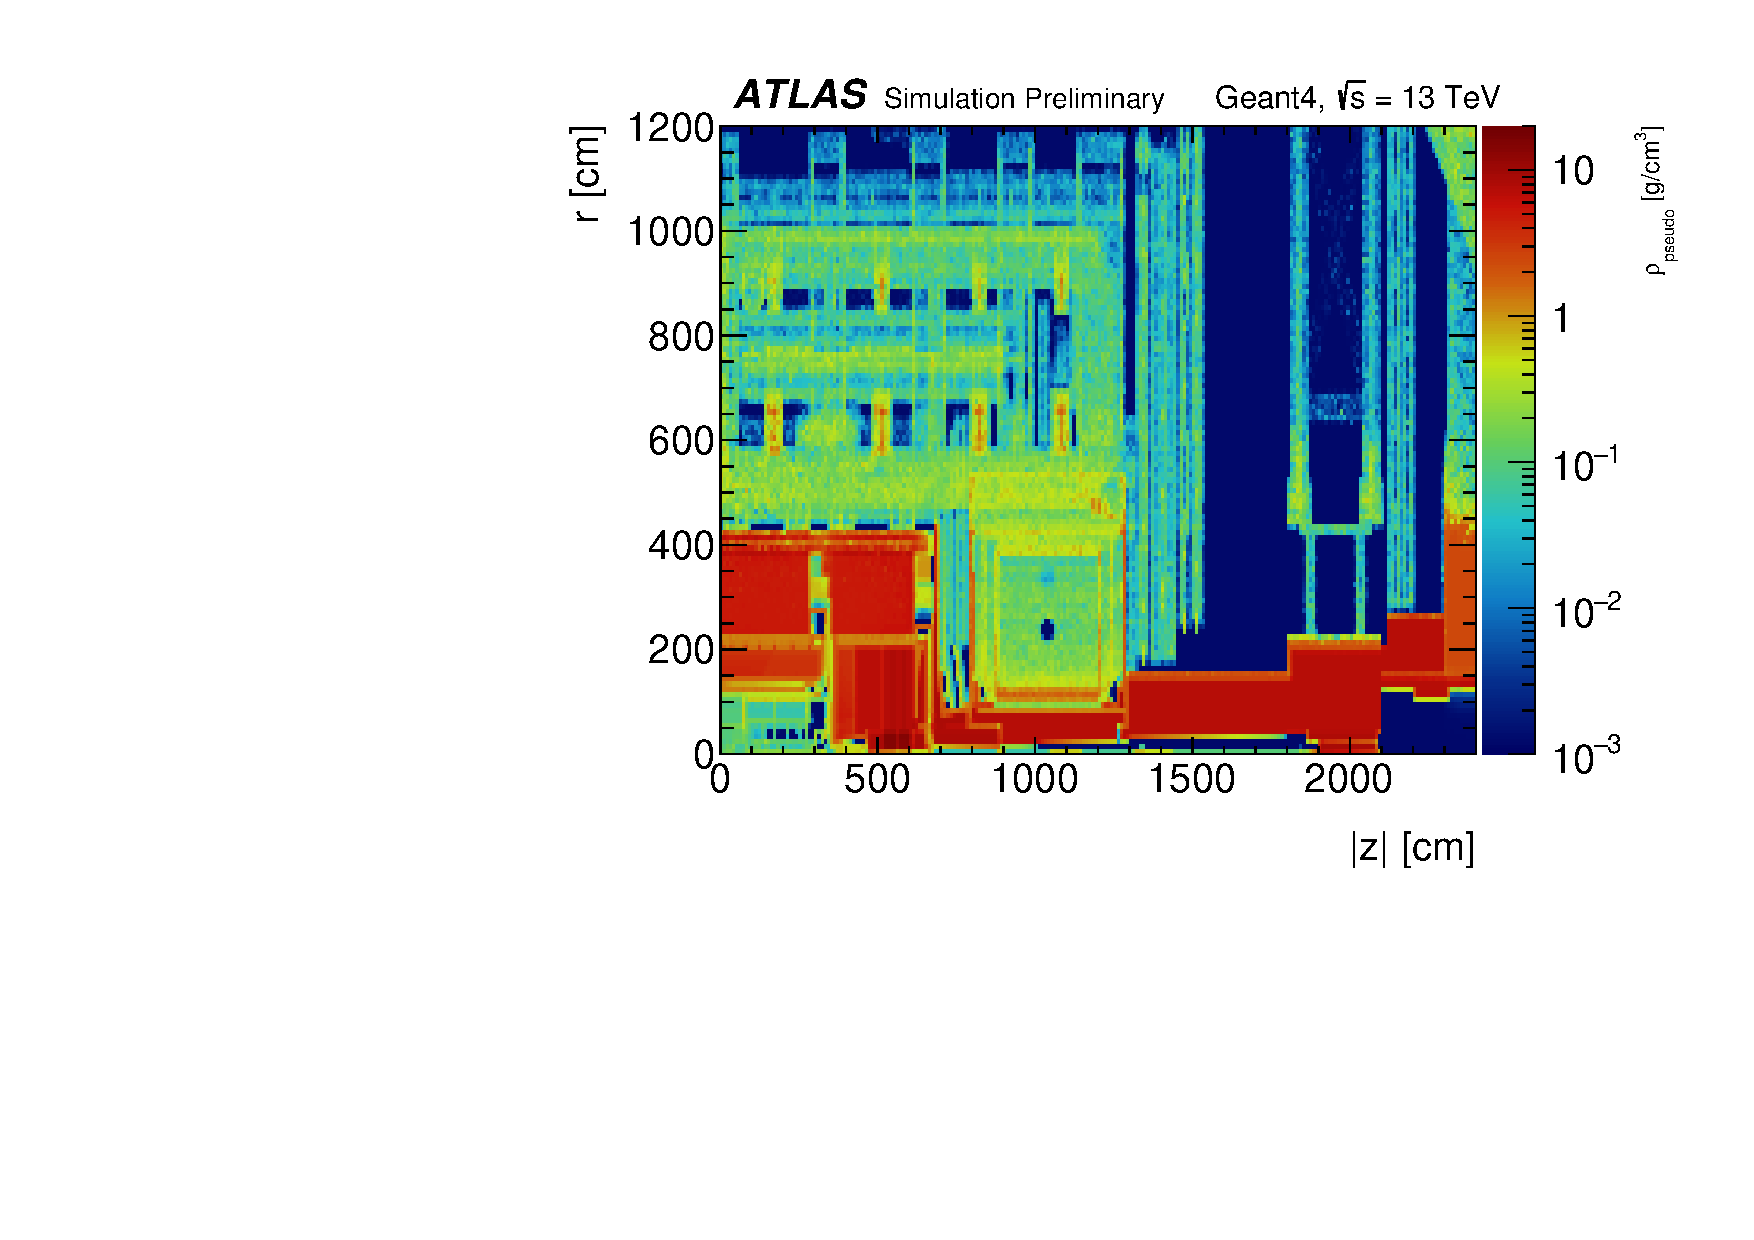
\includegraphics[width=0.8\textwidth]{figures/nsw/atlas_cavern_material_density_sim}
        \caption{
            Simulation of the average material density in materials within a quadrant of the ATLAS cavern.
            %during a minimum bias collision event at $13\,\TeV$.
            %The normalisation of the $z$-axis is arbitrary.
            The forward-calorimeter cryostat, beam-pipe, and shielding ($z\approx 6.8$\,m)
            in front of the Small Wheel experience high energy deposition.
            The largest rates observed by the muon system are those experienced
            by the CSC detectors in the current Small Wheel, which can be seen in the above
            to lie directly behind and above regions of high material interaction.
            Figure taken from Ref.~\cite{ATL-PHYS-PUB-2016-017}.
        }
        \label{fig:cavern_bkg}
    \end{center}
\end{figure}

The NSW will take part in the Level-1 muon trigger by providing
tracking information to aid the TGC-based Level-1 muon trigger logic currently in use for providing
Level-1 muon trigger candidates in the forward region.
The inclusion of such trigger information from the NSW will help to discriminate against
`fake' triggers due to background particles, as illustrated in Figure~\ref{fig:l1mu_rates},
and will also improve the overall muon \pT~measurement in the forward muon trigger which
will enable the Level-1 muon triggers to maintain low \pT-thresholds.
If there were no NSW upgrade, in order to cope with the high rate of Level-1 muon triggers,
the \pT~thresholds of the single-muon triggers would have to be increased from a minimum of $\approx20\,\GeV$
to thresholds well above 40\,\GeV in order to drop the total rate of muon triggers (inclusive of those
in the barrel and end-cap) below the 20\,kHz budget.
Alternatively, the forward muon trigger system could be removed altogether.
In this latter case, all muon triggers would be seeded by Level-1 muon candidates in the barrel only.
Both of these scenarios lead to drastic reduction in physics performance.
Major Higgs-physics goals of ATLAS, for example, would take large hits if either of these
two non-NSW scenarios were enacted.
Increasing the Level-1 muon trigger \pT-thresholds results in a loss in efficiency of more than
30\% for the $Wh,h\rightarrow bb$ process --- a key channel necessary for the observation and study
of the Higgs couplings to $b$-quarks.
A drop in efficiency on the order of 50\% is expected for the same process if the trigger thresholds
are kept low but the forward muon trigger system is removed.
This is illustrated in Figure~\ref{fig:nsw_wh_loss}, both for the $Wh,h\rightarrow bb$ scenario
discussed but also for the $h\rightarrow WW^*$ production channel, an important source of Higgs bosons
in ATLAS.


\begin{figure}[!htb]
    \begin{center}
        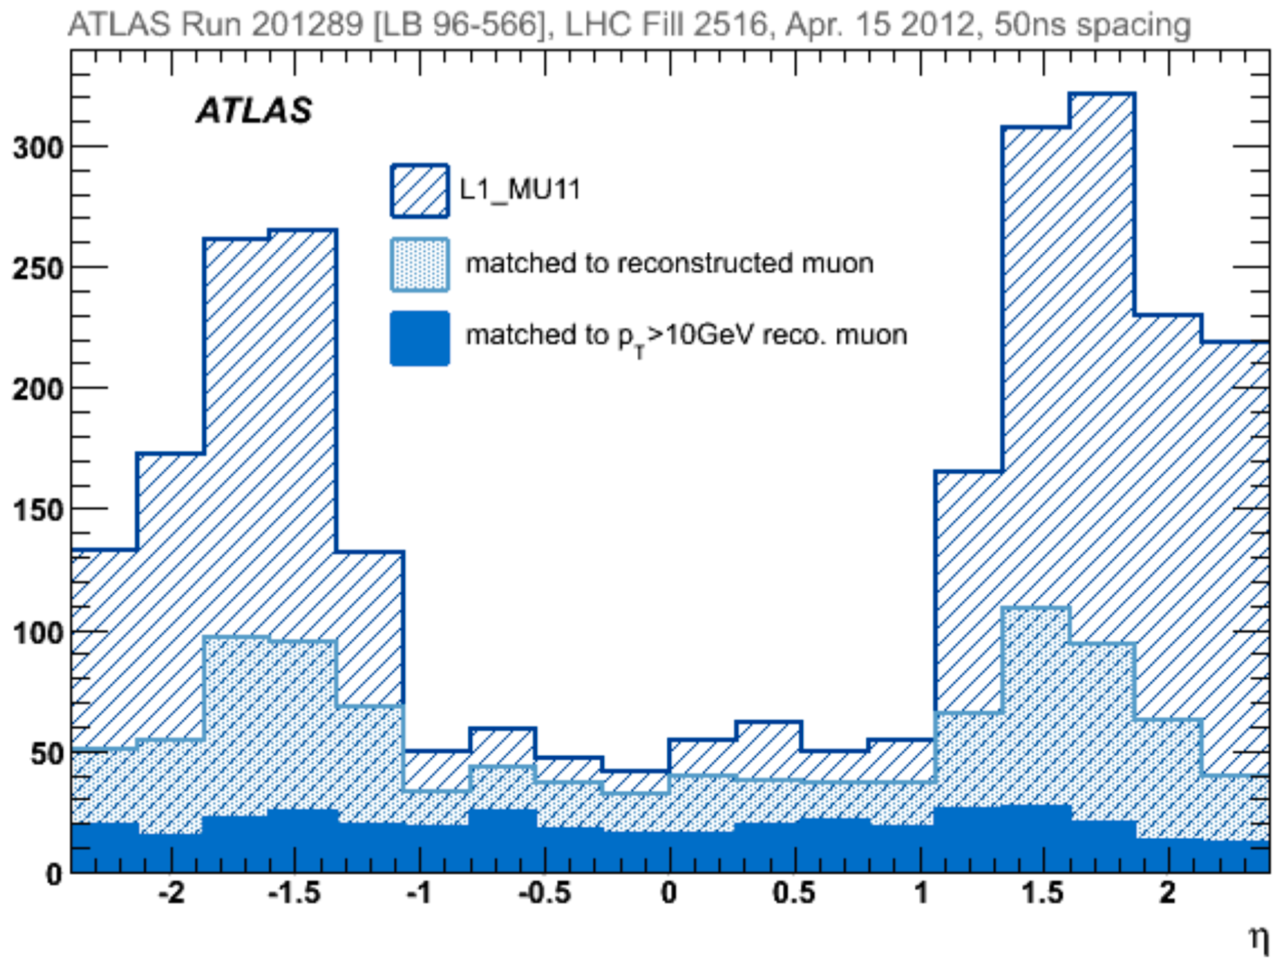
\includegraphics[width=0.47\textwidth]{figures/nsw/nsw_l1mu_rates}
        \raisebox{0.4cm}{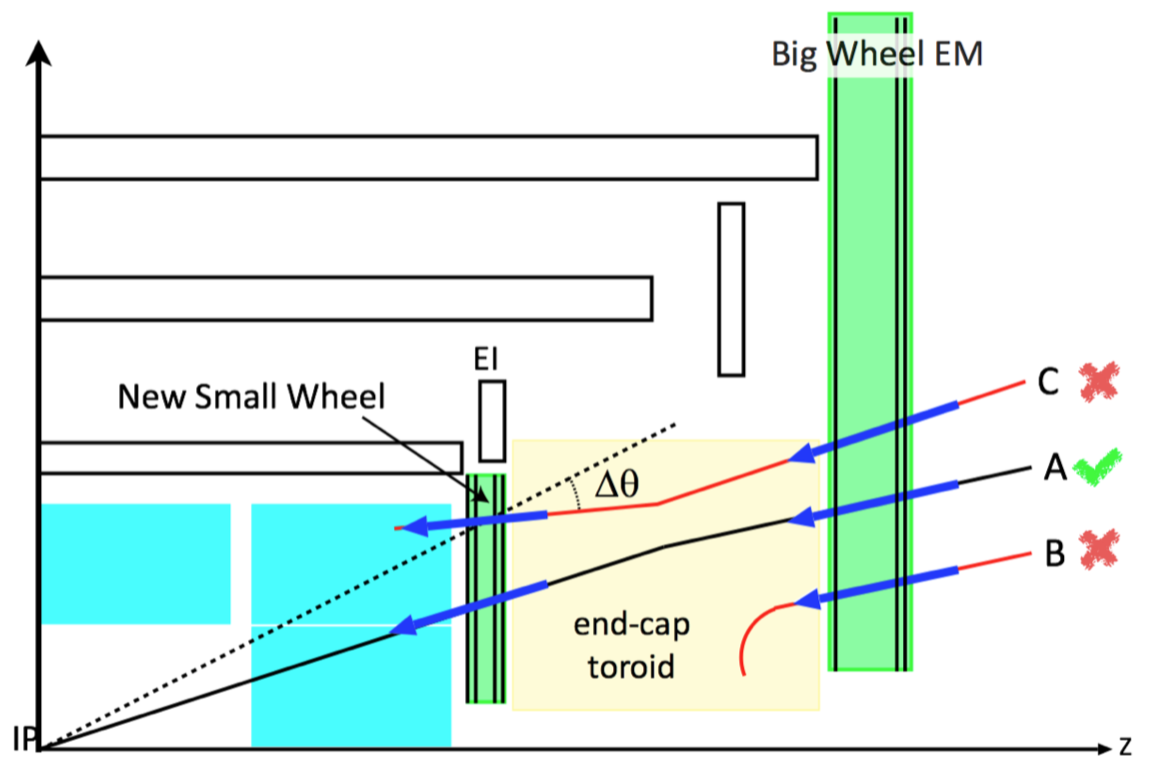
\includegraphics[width=0.5\textwidth]{figures/nsw/nsw_track_principle}}
        \caption{
            Figures taken from Ref.~\cite{NSWTDR}.
            \textbf{\textit{Left}}: Level-1 muon trigger rates as a function of $\eta$. L1\_MU11 refers to the
                rate of the Level-1 accept rate. After requiring that the muon trigger candidates
                responsible for the Level-1 muon trigger firing are matched to a real muon, the
                rate drops significantly, illustrating the rate of `fake' muon triggers in the
                forward muon system.
            \textbf{\textit{Right}}: Illustration of the principle of operation of the NSW trigger system.
                The aim of the NSW trigger is to provide accurate pointing information (via the illustrated $\Delta \theta$ computation) within
                the inner-most muon system to aid the trigger logic of the Big Wheel and thereby reduce the acceptance of `fake' triggers that
                do not have coincident pointing track segments in both wheels.
                With the NSW trigger logic, only the muon trigger candidate labelled `A' will result
                in a Level-1 muon trigger being fired.
                The track candidate `C' (`B') fails to fire a trigger due to non-IP-pointing (missing) track-segments in the NSW,
                characteristic of cavern background particles.
        }
        \label{fig:l1mu_rates}
    \end{center}
\end{figure}

\begin{figure}[!htb]
    \begin{center}
        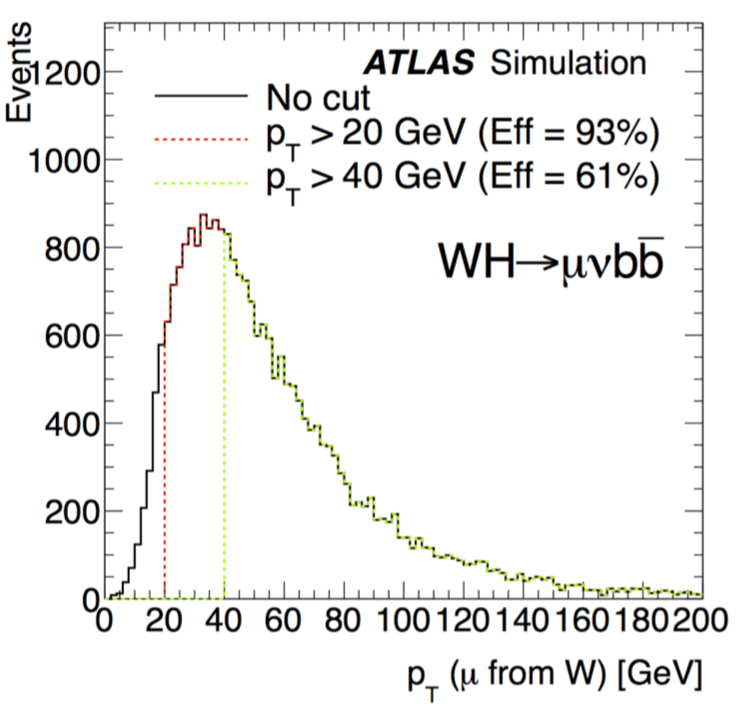
\includegraphics[width=0.4\textwidth]{figures/nsw/nsw_ptmu_wh}
        \raisebox{1.85cm}{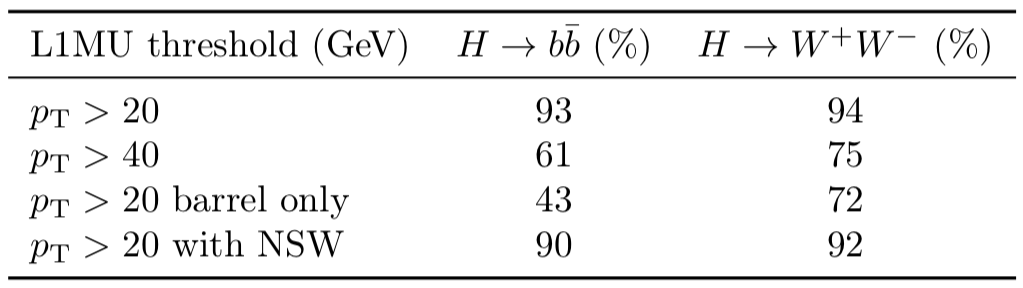
\includegraphics[width=0.55\textwidth]{figures/nsw/nsw_eff_wh_hbb}}
        \caption{
            Figures taken from studies contained in Ref.~\cite{NSWTDR}.
            \textit{\textbf{Left}}: Truth-level \pT~distribution of the trigger-muon in the $Wh$ analysis, showing
                the trigger thresholds and corresponding truth-level selection efficiency of those thresholds.
            \textit{\textbf{Right}}: Selection efficiencies for several trigger-threshold scenarios with and without the NSW
                for the $Wh,h\rightarrow b \bar{b}$ and $h \rightarrow WW^*$ processes.
        }
        \label{fig:nsw_wh_loss}
    \end{center}
\end{figure}

In addition to the trigger performance of the current forward muon system being insufficient
for the foreseen data-taking challenges, the tracking performance of both the MDT and CSC detectors of the current Small Wheel
will also degrade with the increased luminosities.
For example, the MDT detectors are characterised by long signal drift-times that are hundreds of nanoseconds long.
With both these long characteristic drift times and the increased particle rates predicted to occur with the LHC upgrades,
the occupancies that will be experienced by the MDT chambers in the current Small Wheel
will result in significant degradation of their tracking capabilities.
At the high rates expected in the future runs of the (HL-)LHC, the tracking efficiencies
of the MDT chambers will approach 50\% or worse (lower), as illustrated in Figure~\ref{fig:nsw_mdt_track_reco}.
This leads to significant reductions in the capabilities of the inner-most muon stations
in the forward region to provide a third high-resolution muon measurement necessary for the sagitta measurement used for reconstructing
muon momenta.

\begin{figure}[!htb]
    \begin{center}
        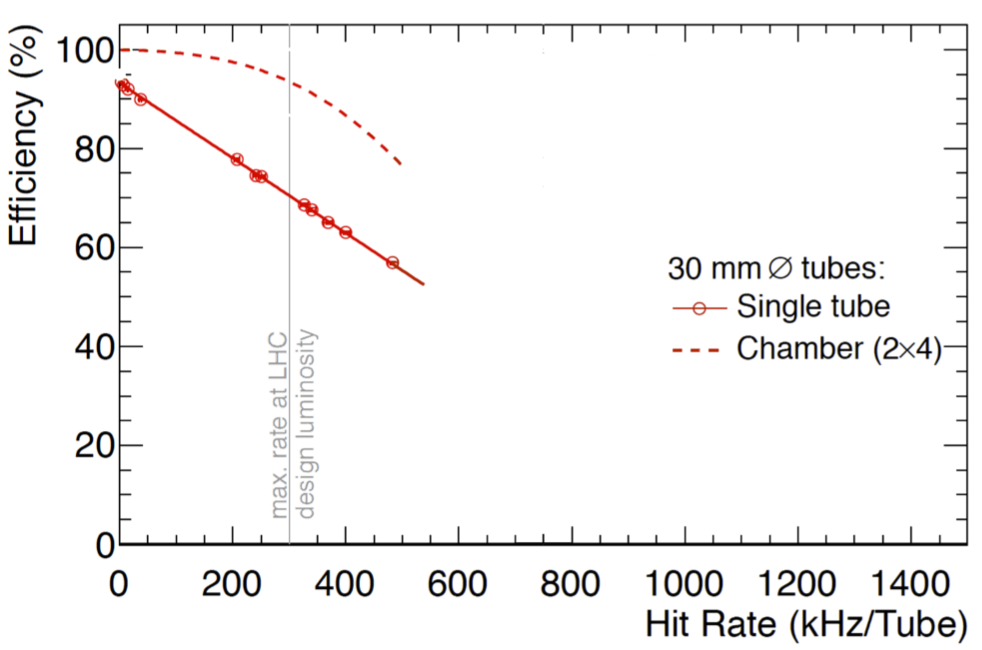
\includegraphics[width=0.7\textwidth]{figures/nsw/nsw_mdt_track_reco_eff}
        \caption{
            Measurements of MDT tube hit (solid line) and track-segment efficiency (dashed-line)
            as a function of tube hit rate.
            The vertical line indicating the maximum LHC rate corresponds to an instantaneous
            luminosity of $1\times10^{34}$cm$^{-2}$s$^{-1}$.
            Figure taken from Ref.~\cite{NSWTDR}.
        }
        \label{fig:nsw_mdt_track_reco}
    \end{center}
\end{figure}
